\section{User Bias for Early Content}

\begin{figure*}[!tb]
\centering
\begin{subfigure}{.3\textwidth}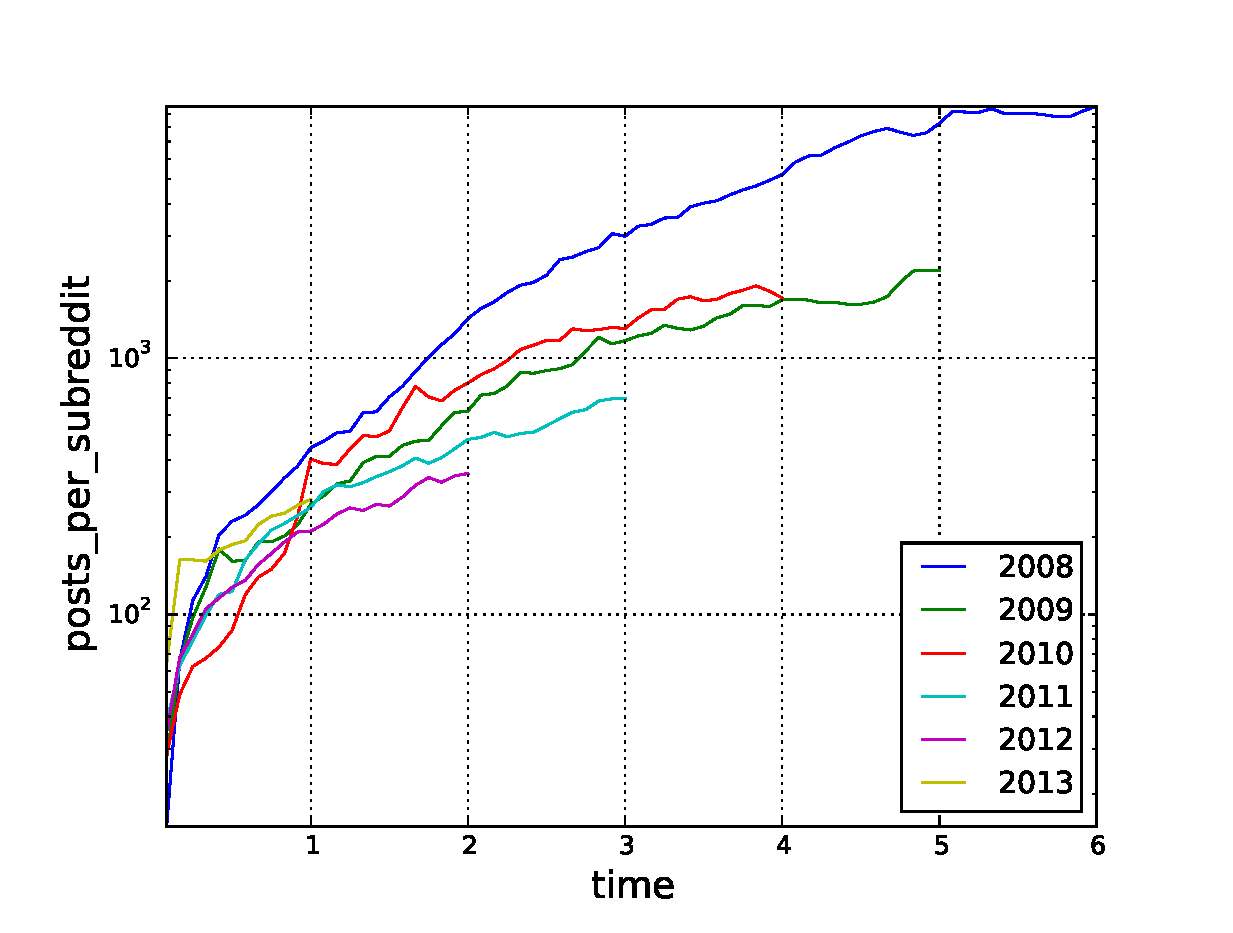
\includegraphics[scale=0.285]{./images/posts_per_subreddit_cohorts.eps}\caption{}\end{subfigure}
\begin{subfigure}{.3\textwidth}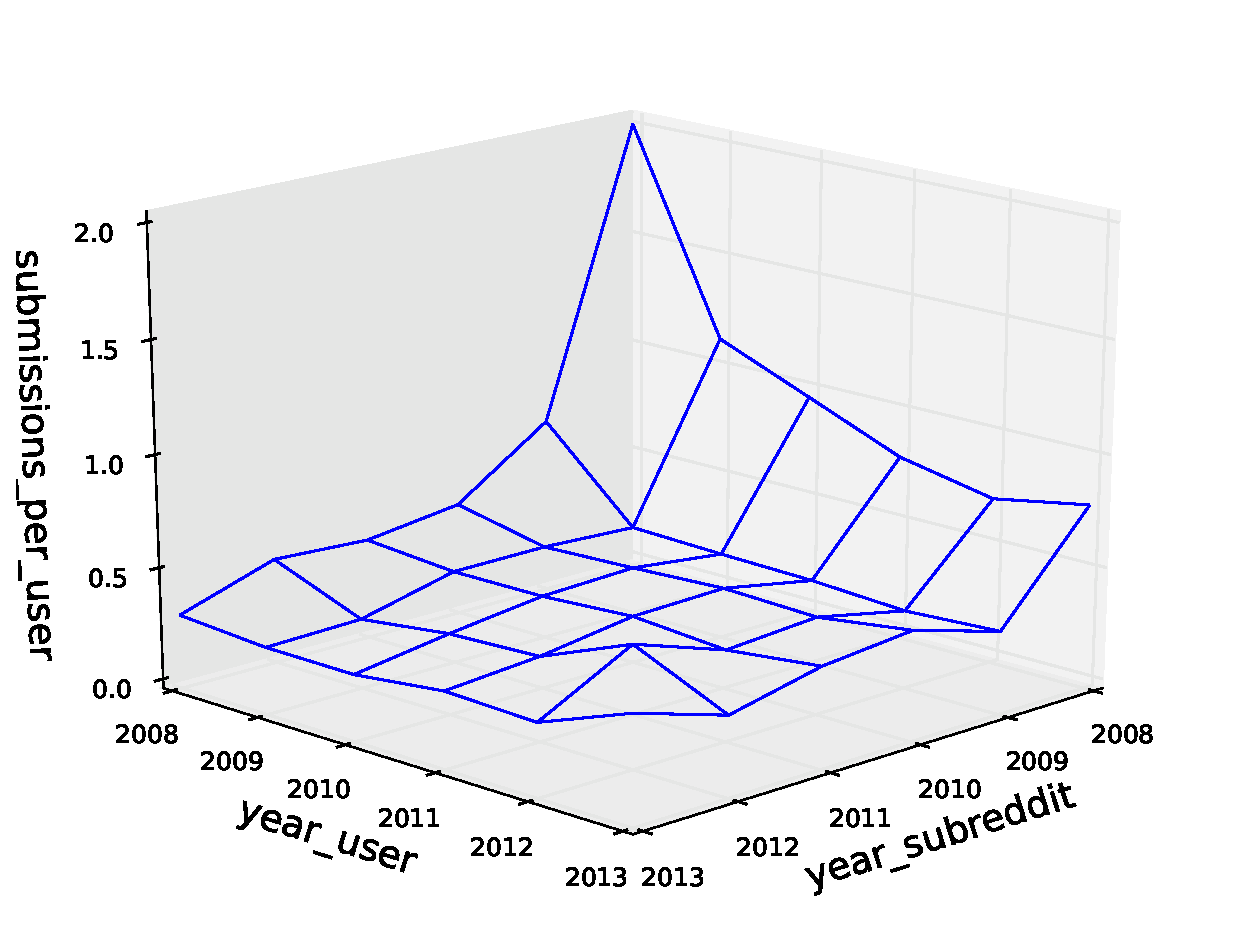
\includegraphics[scale=0.285]{./images/user_subreddit_submissions_cohorts.eps}\caption{}\end{subfigure}
\begin{subfigure}{.3\textwidth}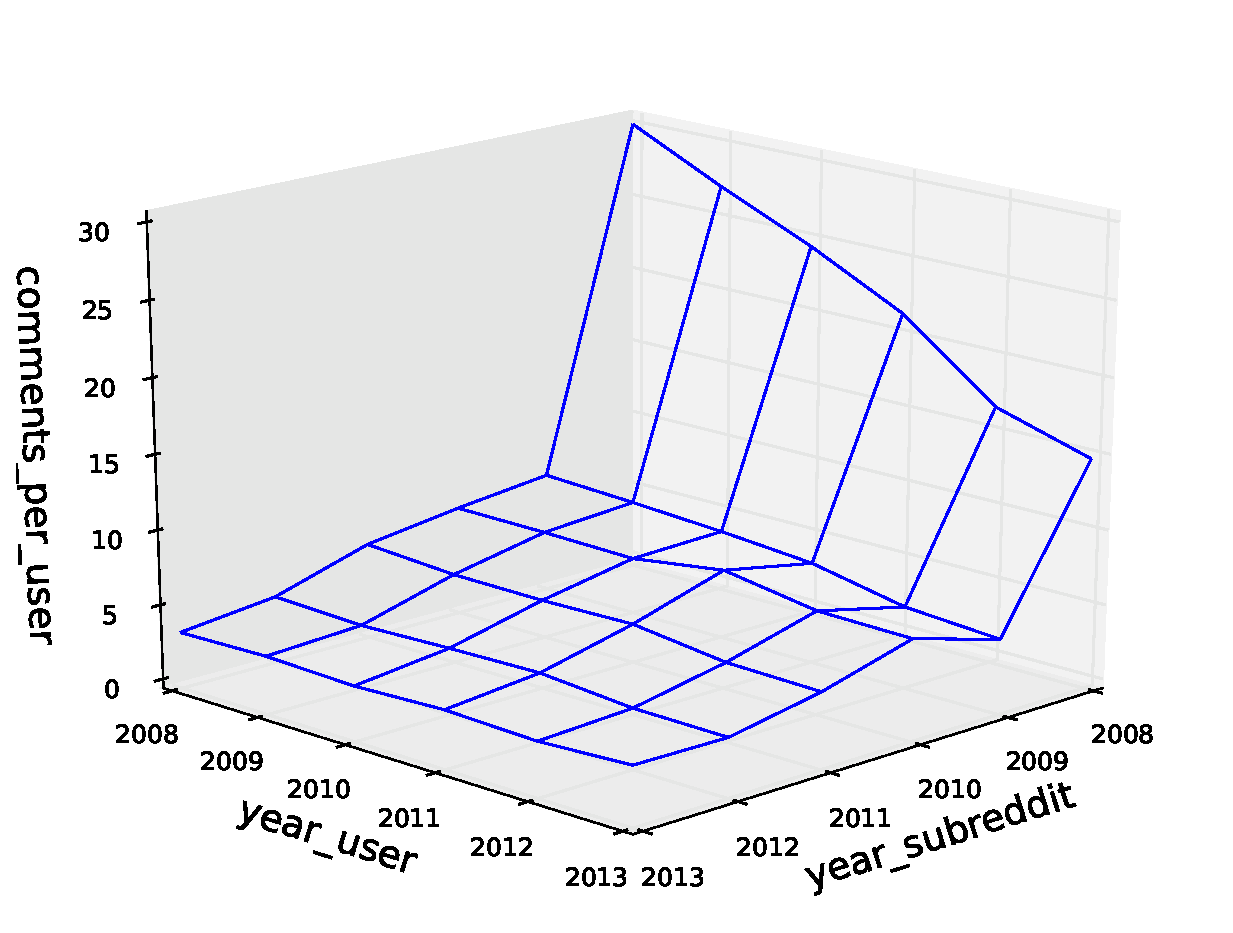
\includegraphics[scale=0.285]{./images/user_subreddit_comments_cohorts.eps}\caption{}\end{subfigure}
\caption{Figure a shows the monthly posts per surviving subreddit cohorted by the subreddit creation date (first post to the subreddit). Figure b and c shows, respectively, the number of submissions and comments per user in reddit for the last three months of 2014, segmented by user creation year and subreddit creation year. Each bin counts the number of comments or submissions based on the user and subreddit creation year and divide by the total number of active users created in that year.}
\label{fig:joint}
\end{figure*}

The cohort a user belongs to has a significant impact to the user posting behavior, but that does not give us a picture of how these users coexist in the current community or the communities evolution on time. An interesting hypothesis that we could imagine is that users from a particular cohort are more interest in the communities from a particular cohort. We now look at the interplay between user and subreddit cohorts. 

Figure \ref{fig:joint}a shows the number of posts in the subreddit-time referential for cohorts on the subreddit creation year. The most striking observation here is how 2008 subreddits are significantly more active than other subreddits for the same survived time. This led us to question what could be the process for this bias. One piece of evidence that we found that can significantly bias the user posting choices are the default subreddits a user is automatically subscribed upon creation \footnote{\url{https://www.reddit.com/r/defaults}}. These subreddits change over time and are said to be ``a set of highly popular communities that the administrators of this site feel would give the average person an interesting first experience'' \footnote{\url{https://www.reddit.com/wiki/reddit_101}}. Even if this set is defined only after the subreddits get popular, there might be a positive feedback that maintains the ``core subreddits'' as the most popular ones. We observe the bias for 2008 when we count each of the default subreddits set over time according to their creation year, seen in Table \ref{tab:defaults}.

\begin{table}[!tb]
\centering
\tabcolsep=0.11cm
\singlespacing
\fontsize{7pt}{8pt}\selectfont
\begin{tabular}{|>{\raggedright\centering\arraybackslash}m{1.5cm}|c|c|c|c|c|c|c|c|}
\hline
 & 2007 & 2008 & 2009 & 2010 & 2011 & 2012 & 2013 & 2014 \\ \hline
December 31, 2009 & 5 & 6 & 1 & - & - & - & - & - \\ \hline
October 18, 2011 & 3 & 14 & 2 & 2 & - & - & - & - \\ \hline
October 19, 2012 & 2 & 16 & 3 & 2 & 2 & - & - & - \\ \hline
July 17, 2013 & 2 & 15 & 2 & 1 & 2 & - & - & - \\ \hline
January 1, 2014 & 3 & 14 & 2 & 2 & 3 & - & - & - \\ \hline
April 19, 2014 & 3 & 13 & 2 & 2 & 2 & - & - & - \\ \hline
May 7, 2014 & 4 & 23 & 6 & 5 & 4 & 7 & 1 & - \\ \hline
\end{tabular}
\caption{Count of subreddits per creation year for each default set of.}
\label{tab:defaults}
\end{table}

Figures \ref{fig:joint}b and \ref{fig:joint}c show a more current picture of reddit. While submissions in Figures \ref{fig:joint}b are in general more skewed towards 2008, it is even more striking that users from 2008 submit even more. This might be due to the fact that these surviving users play a much more central role in these communities (moderators or key contributors) since they are more likely to be there from the start (relative to the total number of users from the cohort that are still active), as we see evidence in Table \ref{tab:mods}. Figures \ref{fig:joint}c show that comments are even more skewed than submissions towards 2008 subreddits. The tendency, however, is of decreasing commenting behavior for the earlier user cohorts (we have seen that users from earlier cohorts are posting less, which justifies this decrease).

%% DC 15: This could be an interesting 
\begin{table}[!tb]
\centering
\tabcolsep=0.11cm
\singlespacing
\fontsize{7pt}{8pt}\selectfont
\begin{tabular}{|l|c|c|c|c|c|c|c|c|}
\hline
 & 2007 & 2008 & 2009 & 2010 & 2011 & 2012 & 2013 & 2014 \\ \hline
Moderators & 757 & 1182 & 2108 & 4085 & 8059 & 9340 & 6868 & 4262 \\ \hline
Percentage & 8.52 & 6.02 & 5.2 & 3.91 & 2.54 & 1.5 & 0.82 & 0.18 \\ \hline
\end{tabular}
\caption{The first lines show the absolute number surviving users that posted as moderators in each cohort. The second line shows the relative percentage to the surviving users for the same cohorts. Were considered active the users in the last three months of 2014.}
\label{tab:mods}
\end{table}
